% Draft Version 1 - Date 16/06/2020
% Draft Version 2 - Date 06/08/2020
% Draft Version 3 - Date 27/08/2020
% Draft Version 4 - Date 14/12/2020
%%CHANGE SUBLEVEL AND micro-structure
% INFO about artificial intelligence and the present situation
\chapter{Introduction}

Cellular micro-structure in materials is one of the structural spatial organization permitting simultaneous optimization of stiffness, strength and overall weight in a given application. Such micro-structures are naturally met in materials like cork, wood, bone and other cellular materials. These cellular properties enable materials in nature to exhibit superior performance for insulation, permeability or to support relatively large loads \cite{ashbyMechanicalPropertiesCellular1983,gibsonCellularSolidsStructure1997}. This has triggered the development of a class of light-weight cellular metallic open foam materials with applications ranging from light-weight energy absorbers for impact loading applications and blast loading in the automotive \cite{banhartManufactureCharacterisationApplication2001}, aerospace \cite{destefanisSelectingEnhancedSpace2006} and other industrial sectors \cite{maEnergyAbsorptionDoublelayer2007,hanssenCloserangeBlastLoading2002} {and more recently in the field of thermal energy storage \cite{digiorgioNumericalAnalysisParaffin2017,liExperimentalNumericalStudies2012}, heat sinks \cite{andreozziNumericalStudyMetal2017,shihExperimentalInvestigationHeat2007} and hydrogen production \cite{villafan-vidalesHeatTransferSimulation2011} among others}. The advancements do not stop here and highly lightweight nanoparticle coated metal foams have been found to be strong enough to absorb shock waves produced by detonations\cite{NanocoatingMakesLightweight}.

\begin{figure}
	\centering
	\begin{subfigure}{0.32\textwidth}
		\includegraphics[width=\textwidth]{foam_sample_alu}
		\caption{}
	\end{subfigure}
	\begin{subfigure}{0.32\textwidth}
		\includegraphics[width=\textwidth]{foam_sample_nicral}
		\caption{}
	\end{subfigure}
	\begin{subfigure}{0.32\textwidth}
		\includegraphics[width=\textwidth]{foam_sample_nicral_int}
		\caption{}
	\end{subfigure}
	\begin{subfigure}{0.38\textwidth}
		\includegraphics[width=\textwidth]{foam_sample_ni}
		\caption{}
	\end{subfigure}
	\begin{subfigure}{0.3175\textwidth}
		\includegraphics[width=\textwidth]{foam_sample_jung}
		\caption{}
	\end{subfigure}
	\begin{subfigure}{0.2825\textwidth}
		\includegraphics[width=\textwidth]{foam_sample_jung_zoom}
		\caption{}
	\end{subfigure}
	\caption{Some typical metallic foams; (a) ERG aluminium foam\cite{andrewsCompressiveTensileBehaviour1999}; (b) Alantum NiCrAl sponge and, (c) the detail of sponge surface\cite{garcia-morenoCommercialApplicationsMetal2016}; (d) NiTECH Nickel foam\cite{badicheMechanicalPropertiesNonhomogeneous2000}; and (e) Celltech Aluminium foam and, (f) its strut cross-section\cite{jungMicrostructuralCharacterisationExperimental2017}.}\label{fig-int-foams}
\end{figure}

Metallic open-cell foams (Figure \ref{fig-int-foams}) can be manufactured indirectly from molds left after thermal treatment of reticulated polymer foams using investment casting, or by electro-deposition  onto a polymeric foam with open cells, which is later removed resulting in hollow struts \cite{banhartManufactureCharacterisationApplication2001}. The resulting foams, in general, follow the morphological characteristics of the polymeric foam from which they are derived. More often than not, they have a complex micro-structure consisting of an interconnected network of ligaments forming along the edges of randomly packed cells that evolve during the foaming process of the polymeric foam \cite{jangMicrostructureOpencellFoams2008}. A near equivalent to this type of material is a reticulated version of the equilibrated liquid foam, like that of soap froth or dry soap foam, where the cells that are near-polyhedral volumes originate from bubbles that are separated by tensioned liquid films. Under conditions of mechanical equilibrium where the surface free energy is minimized, the local foam geometry obeys Plateau's laws \cite{plateauStatiqueExperimentaleTheorique1873,kraynikStructureRandomMonodisperse2003} with constant mean curvature of each face, with three faces meeting at equal dihedral angles of 120\degree\,at each cell edge, and with four edges joining at equal tetrahedral angles of cos$ ^{-1} $(-1/3)=109.47\degree\,at each cell vertex. Since the polymer open-cell foam is obtained by foaming a liquid polymer, the polymer-based mold presents morphologies strongly similar to liquid foams. 

The link between the micro-structure of foams and their physical behavior, such as mechanical, acoustic, or thermal response, has been the focus of many studies considering the varying applicability of these desirable properties. A number of experimental studies addressed this aspect in the literature \cite{jangCrushingAluminumOpencell2009,jangCrushingAluminumOpencell2009a,gongCompressiveResponseOpencell2005,hodgeMeasurementModelingCreep2003,jungNanonickelCoatedAluminum2011}. Along with these, computational models at the micro-structural scale, or homogenization-based multi-scale models, help in building an in-depth knowledge of the relationship between local morphological features and the global behavior of these materials. Considering the higher cost margins induced by the industries due to the low production volumes, the development of efficient computational models becomes important. 

\begin{figure}
	\centering
	\begin{subfigure}{\textwidth}
		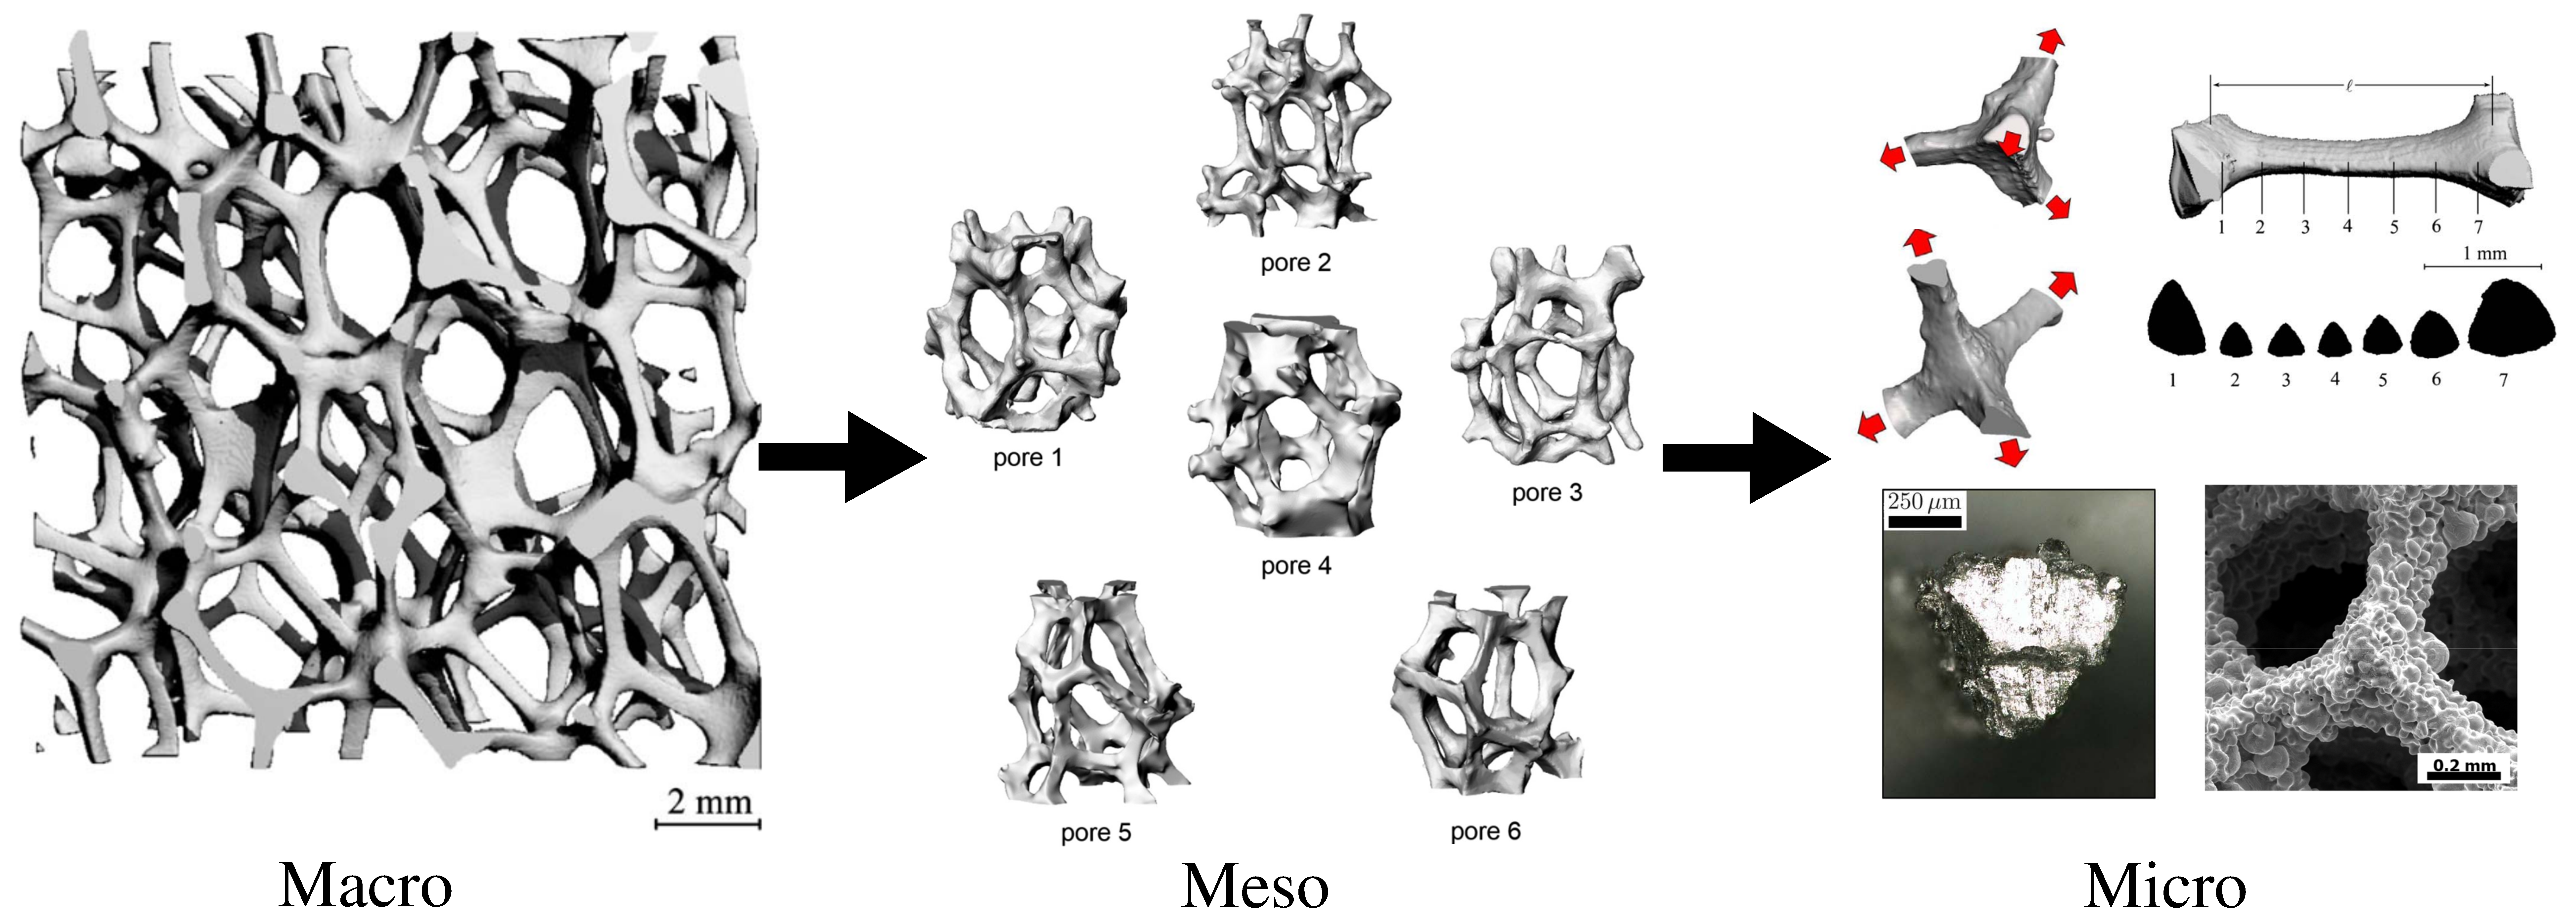
\includegraphics[width=\textwidth]{foam_scale}
	\end{subfigure}
\caption{Hierarchical scale based representation of the material. The units range from cm at macro scale to $ \mu $m at the micro scale. Images sourced from \cite{jangMicrostructureOpencellFoams2008,jungOpencellAluminiumFoams2015}}\label{fig-int-scale}
\end{figure}

Metal foams are micro-heterogeneous materials. It is possible to define the phenomenological description of the material properties using a multiple length scale based hierarchy (Figure \ref{fig-int-scale}). In such a description, the material can be divided into sub-levels that are considered homogeneous in a simulation and the properties at each individual sub-level depend only on the effective inhomogeneities at that sub-level. The sub-level that defines the micro-structure describes the structure of the struts of the foam, the grain size, voids and any inclusions in the strut. As one goes higher, the meso-scale characterizes the length and the thickness of the struts arising due to the varying cross-section and the resultant shape of the pores. At the highest level of homogenization, the macro-scale, several pores of the foam are covered and it is regarded as a continuum where the local damage and deformation mechanisms can not be investigated.

The material response of metallic open foams is characterized by the initial elastic increase in the stress with a small amount of local plastic deformations, followed by a stress plateau due to the successive collapse of the pores in the specimen, and finally a steep increase in the stress due to material densification (Figure \ref{fig-int-sample}(a)). It also becomes necessary to identify the bulk material properties of the individual strut elements so as to not over-estimate the stress-strain response leading to very high stiffness\cite{jungModellingMetalFoams2016}. A study on effective  micro-material properties has been presented in \cite{heinzeExperimentalNumericalInvestigation2018} (Figure \ref{fig-int-sample}) where the authors have identified effective micro-mechanical properties, i.e., the material properties of the struts of aluminium foams using inverse modeling techniques.

\begin{figure}
	\centering
	\begin{subfigure}{0.45\textwidth}
		\includegraphics[width=\textwidth]{only_data}
		\caption{}
	\end{subfigure}
	\begin{subfigure}{0.45\textwidth}
	\includegraphics[width=\textwidth]{foam_pore_samples}
	\caption{}
	\end{subfigure}
	\caption{(a) Experimental observations of the material response of some metallic open foam specimens as observed in \cite{jungMicrostructuralCharacterisationExperimental2017} during uniaxial compression. The zones of (1) elastic regime, (2) plateau regime and (3) densification regime has been labeled. (b) Material response of individual pores as observed in \cite{heinzeExperimentalNumericalInvestigation2018}. }\label{fig-int-sample}
\end{figure}

A numerical study of the material behavior of these open foam micro-structures can be carried out by a well structured computational homogenization scheme that takes the macro scale as a continuous homogeneous media while applying the constitutive behavior of the strut material on the micro-scale. This necessitates the ability to model the micro-structure by taking into account the various complexities that are observed in the physical foams that are in use. Idealization of the micro-structure by assuming it to visually be similar to various geometrical patterns assembled in a predictive or a periodic manner is an easy way to obtain the basic elastic properties of the foam structures. However, it is better if such models can statistically represent the general foam features by taking into consideration as few assumptions as possible to avoid the accumulation of errors resulting due to these assumptions on the macro behavior of the material model. These complexities can be obtained through the generation of tessellations based on random spherical packings.

Nevertheless, a detailed representation of the micro-structure often leads to an overwhelming computational cost. In recent times, significant progress has been done to reduce the computational cost of these computational homogenization procedures. The optimization can be achieved by either reducing the model complexity in what is known as reduced order modeling, but at the expense of complex numerical analysis, or by the advanced tools made available thanks to the progress in machine learning approaches like artificial neural networks. 

\section{Micro-structure representation}

A model structure, with repeated calculations with varying model parameters, allows investigating the changes in the overall material properties associated with changes in the micro-structure. 

In this regard, 3D characterization and modeling of real structural foams using computer tomography (CT) images can provide significant insight into the sample structure. These images can then be discretized and studied using finite element method (FEM) simulations \cite{veyhlFiniteElementAnalysis2011,fiedlerMCTbasedFiniteElement2012,fiedlerComputedTomographyBased2009}. Yet, this remains a daunting task since characterizing all the samples requires both time and processing capacity, thus restricting the analysis to smaller samples requiring user-assisted analysis of the images \cite{montminy3DStructureReal2004}. 

Another reconstruction methodology based on CT scan images has been presented in \cite{leblancAnalysisOpenFoamUnderPreparation} where the individual pores of the foam samples have been embedded with ellipsoids and polyhedrals. This method, while being computationally cheaper than the standard watershed algorithm\cite{lautensackFittingThreedimensionalLaguerre2008}, is also capable of implicitly capturing the anisotropy present in the foam samples that could be generated due to the manufacturing method used. 

Idealization of the geometry with the help of deterministic models such as the Kelvin\cite{thomsonLXIIIDivisionSpace1887} or the Weaire-Phelan\cite{weaireCounterexampleKelvinConjecture1994} was developed to obtain numerically derived models. To overcome the inability of these numerical models to capture the local variations occurring in the foam samples, random Laguerre tessellations generated by non-overlapping sphere packings were presented in \cite{redenbachMicrostructureModelsCellular2009}. A completely numerical approach based on sphere packing algorithms and an eventual surface minimization based approach to extract the foam micro-structure has been presented in \cite{kraynikStructureRandomFoam2004}. 

A novel approach was presented in \cite{sononAdvancedTechniquesGeneration2014} in which the authors make use of level sets and implicit surfaces represented by the direct and indirect usage of the level sets that are generated by points and arbitrarily shaped surfaces. From its use as a random packing generator to applications in textile fiber orientations, the level sets have the capability to represent various morphologies including cellular materials. With the help of discrete grids of points, the morphologies can be extracted as statistically Representative volume elements (RVE) that can then be used to study and analyze virtual models undergoing complex loading. The presence of distance functions and level sets enables the extraction of well defined and morphologically representative models of open foam structure that can be used conveniently as a micro-model in various analysis tools.

Any modeling tool that enables researchers to obtain better geometries of physical objects needs to be quantitatively as well as qualitatively analyzed. There are several studies in literature that look into the mechanical properties as well as the micro-structural geometries of open foam made of various materials, ranging from polyethylene, aluminum, titanium alloys to coated hybrid metal foams\cite{zhouInvestigationMicrostructureStrength2002,zardiackasStructureMetallurgyMechanical2001,sypeckStructureDeformationAluminum1998,stormInfluenceCurvedStruts2015,pangSynthesisMechanicalProperties2012}. To establish the usefulness of the geometry generator, it becomes necessary to compare the geometry of the randomly generated model to other existing modeling tools as well as physical studies on experimentally generated foam samples. In \cite{jungMicrostructuralCharacterisationExperimental2017}, the authors present a detailed analysis of the effect of the pore size on the material behavior while in \cite{heinzeExperimentalNumericalInvestigation2018}, this study has been conducted on single pore samples of the foam along with a study based on reconstruction of the geometry from computer tomography (CT) scan images and photogrammatry, or reconstruction based on photographs.

Finally, in order to use the extracted geometries in a well structured multi-scale computational homogenization strategy, the RVE geometry needs to be discretized into finite elements. An approach to generate conformal meshes from implicit surfaces was presented in \cite{ehabmoustafakamelIntegratedApproachConformal2019} which utilizes basic triangulation techniques provided by standard meshing tools and generates a refined mesh while maintaining the topological conformity. This mesh methodology will be adopted in the sequel.

\section{Multiscale methods}
The application of material characterization to a very detailed level is helpful in bridging the knowledge gaps that exist currently in the understanding of overall behavior of cellular materials and complementing real experiments with virtual testing means is very much the way forward in the field of study and analysis of complex micro-structures. Considering the fact that cellular materials exhibit complex mechanical behavior due to various issues like size-effect\cite{andrewsCompressiveTensileBehaviour1999} or localization phenomena due to micro-buckling of thin components like cell struts\cite{jangCrushingAluminumOpencell2009}, which strongly influences the structural stiffness, the study of the behavior of the cellular materials needs to be properly organized. In this regard, the detailed geometry of the structure after extraction can be studied using finite element formulations by direct numerical simulation (DNS) at the microscopic scale \cite{mangipudiMultiscaleModellingDamage2011,gibsonCellularSolidsStructure1997} which could possibly lead to a solution that needs a large number of unknowns to be considered. Another approach considers the cellular structure as a continuous medium on which a phenomenological model can be applied\cite{forestContinuumModelingStrain2005} called the macroscopic approach. This method while being efficient can not account for the complex geometries of the micro-structure. Also, the evolution of the micro-structure during the loading phase will not be captured. This brings attention on combining the two methods, where two separate Boundary Value Problems (BVP) are defined at two separate scales in a method also known as FE$ ^2 $. 

However, because of the complexities in the micro-structure, \fee simulations cannot be envisioned to study lightweight structures because of the current limitations in computational resources. 
%{A lot of times}, due to limitations of computational power necessary for the data processing of images extracted by standard CT scanners, one can only expect a very small sample of the foam to be imaged. This data may not always be sufficient to conduct an efficient RVE based computational analysis of the behavior and to address these kinds of issues, \cite{cottereauStochasticdeterministicCouplingMethod2013} discusses algorithms to couple a deterministic model to a random stochastic RVE based on a weak energy coupling operator. This model is able to circumvent the bias observed due to over-constraints introduced by the boundary conditions on the RVE.
At this juncture, one can make use of the computational tools developed in the software industries as well as the advancements in the electronics industries to find suitable solutions to reduce the computational cost and time involved in the classical multiscale methods. Reduced order basis and machine learning solutions can then be considered as an efficient surrogate in the multiscale computational homogenization process.

\section{Data driven analysis}

It is a consistent challenge to improve the efficiency of solvers that are used to analyze various behavioral traits of complex micro-structures, all while increasing the fidelity of the same micro-structure representation. The same problem recurs with the use of FE$ ^2 $ approaches where, to avoid the loss of generality, an embedded micro-model at each macroscopic integration gauss point can lead to extreme increase of the processing power needed. 

Model reduction strategies based on non-uniform transformation field analysis developed on the basis of principal component analysis\cite{michelModelreductionApproachMicromechanics2016,michelNonuniformTransformationField2003,jolliffePrincipalComponentAnalysis2014} or proper orthogonal decomposition\cite{yvonnetReducedModelMultiscale2007} have tried to circumvent the complexities, but at the expense of extensive \textit{a priori} simulations that are necessary to capture the complex behavior. Reduced order methods such as the manifold learning methods based on isomaps have also been studied for heterogeneous materials\cite{bhattacharjeeNonlinearManifoldbasedReduced2016}. However the applications of these methods for dependent plastic materials can be more challenging, either because of the time required to evaluate the local constitutive laws for the former family, or due to the difficulty to frame the history dependency for the latter ones.

To reduce the burden on the processors and to not give away the efficiency, it would be interesting to look towards the efforts made in data mining and artificial intelligence fields and go through various data driven models as surrogates or supporting tools in FE$ ^2 $ analysis which could be capable of dramatically accelerating the scheme.

A distance-minimizing based scheme has been presented in \cite{kirchdoerferDatadrivenComputationalMechanics2016} that can be construed as the beginning of a renewed interest on data driven solvers to accelerate multi-scale analysis. The scheme presented tries to find a corresponding point in the material dataset that tries to minimize the error while trying to satisfy the essential boundary conditions, avoiding the need for constitutive material model. Moving on to large deformations, material data has been presented in a lower dimension and a hidden constitutive manifold is attempted to be solved by following an adaptive search direction\cite{chinestaDataDrivenComputationalPlasticity2017}. In \cite{bessaFrameworkDatadrivenAnalysis2017}, the authors have developed a data-driven computational framework that approximates the relationship between the key descriptors of each design and the quantities of interest to address the issue of high dimensionality of the problems. 

The current level of progress achieved in the artificial intelligence has led to a very focused interest on machine learning based models, such as artificial neural networks (ANN) and deep learning, with respect to their applicability to study the mechanics of materials\cite{bessaFrameworkDatadrivenAnalysis2017,ghaboussiAutoprogressiveTrainingNeural1998,ungerNeuralNetworksMaterial2009,wangMultiscaleMultipermeabilityPoroplasticity2018}. ANNs in specific, also known as connectionist systems, are computing systems that are vaguely inspired by the biological neural networks\cite{chenDesignImplementationCloud2019}. These systems can be trained to ``learn" particular tasks without any specific programming with task-specific rules. A simple example, from the field of image recognition, is when a set of images manually labeled with ``car" and ``no car" can be trained to predict whether a car is present or not in a new image without any specific programming to recognize car specific features like tires, doors, or the shape of the car. The ANNs can do this simply by generating identifying characteristics from the examples that they process.

However, it is very necessary to know beforehand that the data driven tools are developed depending on the specific problem, and may not work very well beyond the original sampling space, in particular for different material laws and loading paths. Significant work is also necessary to tackle history dependency, physical invariance and conservation laws as the models do not consider the physics of the behavior and simply predict based on mathematical and statistical calculations.

ANNs have the advantage of being versatile in their design and thus form a very useful tool in the quest to surrogate efficiently an FE$^2$ analysis. Ranging from a simple multi-layer perceptron to deep neural networks\cite{haykinNeuralNetworksLearning2009}, ANNs have changed the modern digital computing age, and the abundance of available data on various aspects of human life through simple click of a smartphone button, influencing the technology that brings humanity various conveniences like linguistic translation to assisted-driving. Unfortunately, the abundance of data required to train the ANN cannot be extracted experimentally. But the availability of modeling tools has presented a curious case of an abundance of virtual data that can be used instead. It then becomes imperative that the virtual data used to train the ANN models are of satisfactory quality. The non-linearities present in complex micro-structure ensures that the training process of the virtual data is not a cakewalk and needs constant studying so as to not generate a myriad of garbage predictions\cite{rochaMicromechanicsbasedSurrogateModels2020}.

When it comes to applications of ANNs on fields related to mechanics, there have been some considerable recent works that can be found in literature. ANNs have been used to replace some of the parts of  material constitutive  laws in \cite{furukawaImplicitConstitutiveModelling1998,furukawaAccurateCyclicPlastic2004,wangMetamodelingGameDeriving2019}, and as FE surrogates in \cite{lefikArtificialNeuralNetwork2003,hashashNumericalImplementationNeural2004,zhangUsingNeuralNetworks2020}. In \cite{wuBayesianInferenceNonlinear2020}, the authors have used ANNs to substitute complex material computational homogenization constitutive laws in order to obtain an accelerated computational scheme in the context of the Bayesian inference of the micro-scale parameters.

Expanding this knowledge to \fee analysis can be done in various ways. Simple sequential feed forward networks (FNNs) have been found to be quite useful in their role as surrogates in computational homogenization procedures, as can be found in \cite{leComputationalHomogenizationNonlinear2015,bessaFrameworkDatadrivenAnalysis2017} where the strain energy density surface has been approximated, or in \cite{fritzenOntheflyAdaptivityNonlinear2019,ungerCouplingScalesMultiscale2008,settgastHybridApproachSimulate2020} where the stress-strain responses have been approximated. Specifically in \cite{settgastHybridApproachSimulate2020}, the micro-scale plastic strains have been used as state variables updated at each loading step in combination with an FNN. However, in cases like elasto-plasticity, where history dependent plasticity is induced in complex micro-structures, it may not be easy to define these state variables.

With the aim of accounting for history dependency, in \cite{ghavamianAcceleratingMultiscaleFinite2019}, recurrent neural networks (RNNs), specifically long short term memory (LSTM) cell based networks were used to study 1D elasto-visco-plastic cyclic loading conditions. In \cite{wuRecurrentNeuralNetworkaccelerated2020,gorjiPotentialRecurrentNeural2020}, gated recurrent unit (GRU) cell based networks have been used to represent micro-scale responses of 2D RVEs under non-proportional loading and have been found to be more efficient.

\section{Objectives of the present work}

In this work, new methodologies have been developed in order to study the response of open foam metallic structures. 

Firstly, an effort has been put to represent open foam morphologies, keeping in mind the geometric constraints and model refineness using level sets and distance functions. Particular focus has been put on capturing the intricacies of the strut geometry so as to capture deformations like buckling that influence the overall foam properties. The generated RVE can then be used in a multi-scale analysis as the micro-scale geometry that influences the macroscopic homogenized behavior of the RVE. \red{A methodology to develop sharp edges of the open foam struts has been presented with the help of a multiple level-set based approach. The entire tool has been presented such that both random geometries as well as reconstruction of geometries based on CT scans of open foam physical samples can be conducted.}

To validate the accuracy of the models thus developed, a study has been done by comparing the virtual behavior with that of an actual sample, the computed tomography (CT) scans of which have been used as a seed to generate the RVE. Various tools and techniques that have been used to generate these morphologies are explained in detail. 

To speed up the computational efficiency of the multi-scale analysis of such complex geometries, various data-driven models have been studied. Considering 2D structures as proof of concept, a surrogate has been developed that uses ANNs to boost up the performance of computation from simple architecture. Relevant mechanical theory to obtain the aforementioned efficiency has been sketched out in detail to demonstrate the ability of the surrogate. The problems faced and the possible solutions to overcome these problems have also been studied and mentioned here so as to present an accurate picture of the current state of art, its abilities and its shortcomings.

This work is organized as follows:
\begin{itemize}
	\item In Chapter \ref{chap-ch}, \textit{\titlech}, a computational homogenization scheme based on multi-scale analysis is presented that uses a first order based approach to formulate the relevant theory behind the homogenization process. Use of relevant boundary conditions to formulate the BVP has been discussed. 
%	In particular, a description of a self-consistent coupling algorithm is also presented where the elasto-plastic model applied on the RVE is coupled to an embedded media that behaves based on a polynomial hyper-elastic based model.
	\item In Chapter \ref{chap-of}, \textit{\titleof}, a distance neighbor based packing algorithm is developed that can implicitly generate morphologies. Functions necessary to extract open foam morphologies from the distance functions generated are presented along with various tools necessary to extract strut geometries. An efficient method to reconstruct morphologies from CT scans is also presented and tools necessary to post-process these image-based morphologies are discussed. Finally, the extraction of finite element models based on the contours generated by the various distance fields are presented.
	\item In Chapter \ref{chap-res}, \textit{\titleres}, discussions on the morphologies extracted from the distance neighbor based algorithm are presented. Statistical validation of the morphologies along with the study of their mechanical behavior is discussed. A virtual model extracted based on this work is compared with a physical model extracted from CT scan images along with discussions on their respective effectiveness and shortcomings due to application of various boundary conditions.
	\item In Chapter \ref{chap-nn}, \textit{\titlenn}, a study on ANNs is developed that details the current state-of-the-art in the field of computational homogenization and data-driven solvers. Some possible surrogate neural networks are studied and compared that can be used in large scale prediction of virtual behavior and possibly in the future on experimental behavior. ANN models based on a combination of Feedforward Neural Networks (FNN) and Recurrent Neural Networks (RNN) are presented to conduct material analysis with history-dependent behavior that can be implemented in an FE$^2$ setting.
\end{itemize}

\section{Contributions}

The contributions of this work are as follows:
\begin{enumerate}
	\item Starting from works presented in \cite{sononAdvancedApproachGeneration2015}, a geometrical tool has been developed that can model the micro-structure of open cell foams using distance fields and level sets taking into account various features like the struts cross-section evolution, etc. \red{A methodology has been developed that takes into account multiple level sets calculated as a function of different distance fields and generates sharp edges corresponding to the open foam struts which was missing. The developed tool then refines the surface mesh extracted from these modified level sets and generates a tetrahedral mesh form of the geometry. Also, the implicit extraction of strut geometry variations is described in detail.} The resulting micro-structures have been validated through statistical indicators like the number of pores, faces, etc. The homogenized material behavior of the foam model thus generated have been statistically validated against experimental observations. 
	\item An efficient way to reconstruct the geometry of open foams from CT scans has been developed that can also store the required distance fields implicitly. A computationally cheaper method to obtain inclusion packing from CT-scan has been presented in \cite{leblancAnalysisOpenFoamUnderPreparation} which has been used as the base packing to develop distance fields. \red{Thus, starting from CT-scan images, an extension has been developed that builds distance fields and level sets that can then be used to build back the open foam geometry in the form of tetrahedral mesh.} The developed foam model behavior has been compared with the corresponding experimental observations to understand the utility of the reconstruction strategies. 
	\item A machine learning study has been conducted and various neural network based models have been tested as efficient surrogates during the computational homogenization process. \red{In this regard, various artificial neural networks like feedforward neural networks and recurrent neural network modules are prepared, trained to predict homogenized behavior of open foam morphologies and tested against direct numerical solution based results.} The developed models have been compared with the traditional FE methods at the micro-scale to obtain the material behavior and understand the complexities and the shortcomings involved in data driven approaches with respect to computational mechanics.
\end{enumerate}

\section{Publications}

This work has directly resulted in the publication of the following article in peer reviewed journal as main author:
\begin{itemize}
	\item N. G. Kilingar, K. Ehab Moustafa Kamel, B. Sonon, T. J. Massart, and L. Noels.
	Computational generation of open foam representative volume elements with morphological control using distance fields. 
	European Journal of Mechanics - A/Solids,
	page 103847, September 2019;
\end{itemize}
and as co-author:
\begin{itemize}
	\item L. Wu, V. D. Nguyen, N. G. Kilingar, and L. Noels. 
	A recurrent neural network accelerated multi-scale model for elasto-plastic heterogeneous materials subjected to random cyclic and non-proportional loading paths.
	Computer Methods in Applied Mechanics and Engineering, 
	369:113234, September 2020.
	\item C. Leblanc, N. G. Kilingar, A. Jung, K. Ehab Moustafa Kamel, T. J. Massart, E. Bechet, and L. Noels. 
	Development of open-foam morphologies by reconstructing CT-scan images.
	In preparation.
\end{itemize}
This work has been presented at the following international conferences:
\begin{itemize}
	\item Nanda Gopala Kilingar, Ludovic Noels, Karim Ehab Moustafa Kamel, Bernard Sonon,
	and Thierry Jacques Massart. Generation of open foam RVEs with sharp edges using Distance fields and Level sets. In ECCOMAS Thematic Conference on Computational modeling of Complex Materials across the Scales - CMCS 2017, November 2017.
	\item Nanda Gopala Kilingar, Ludovic Noels, Karim Ehab Moustafa Kamel,
	and Thierry Jacques Massart.
	Generation Of open foam RVEs
	With Strut Variations Using Distance Fields And Level Sets.
	In
	The 9th International Conference on Computational Methods
	(ICCM2018), June 2018.
	\item Nanda Gopala Kilingar, Ludovic Noels, Thierry Jacques Massart, Karim Ehab
	Moustafa Kamel, Bernard Sonon, Christophe Leblanc, and Anne Jung. Data
	driven computational analysis of open foam RVEs. In Computational Methods in Multiscale, multi-uncertainity and multi-physics problems conference
	CM3 2019, July 2019.
\end{itemize}
%\textit{}